% MemInterfere: ACL/EMNLP format paper
% Compile with: pdflatex paper.tex && bibtex paper && pdflatex paper.tex && pdflatex paper.tex

\documentclass[11pt]{article}
\usepackage{acl}
\usepackage{times}
\usepackage{latexsym}
\usepackage{amsmath}
\usepackage{amssymb}
\usepackage{booktabs}
\usepackage{graphicx}
\usepackage{multirow}
\usepackage{hyperref}
\usepackage{appendix}
\usepackage{xcolor}

\title{Skill Library Interference in LLM Agents: \\ Mostly Harmless, Sometimes Costly}

\author{
  % Author names blinded for review
  Anonymous Authors \\
  Anonymous Institution
}

\date{}

\begin{document}

\maketitle

\begin{abstract}
Large language model (LLM) agents rely on skill libraries---collections of tool descriptions---to select and invoke appropriate tools. A common concern is that \textit{skill library interference}---the presence of near-duplicate, stale, or conflicting skill descriptions---degrades tool selection accuracy. We present MemInterfere, a systematic investigation of this hypothesis across 4 models, 80 tasks, and 5 conditions totaling 4,800 runs (excluding 3 ambiguous tasks; 95.8\% clean vs.\ 94.6\% interference). Surprisingly, interference does \textbf{not} significantly degrade selection accuracy: the difference is 1.2 percentage points (Cohen's $d = 0.06$, $p = 0.26$), and a logistic mixed-effects model confirms this (OR $= 0.77$, $p = 0.28$). Equivalence testing at $\pm$3pp (TOST $p = 0.035$) confirms the effect is smaller than a minimal clinically meaningful difference, though we note this bound is informed by task ceiling effects (83\% of tasks show identical outcomes across conditions). On harder tasks (68.7\% baseline), interference paradoxically \emph{improves} accuracy by 4.9pp ($p = 0.023$), though this finding requires replication with pre-registration. A revised oracle condition (99.8\% accuracy) reveals the task is fundamentally about retrieval, not invocation. The significant costs of interference are secondary: confidence drops of 0.6--1.8pp ($p < 0.01$) and token cost increases of 2.1--2.4$\times$.
\end{abstract}

\section{Introduction}

LLM agents are increasingly deployed with access to tool libraries containing dozens to hundreds of skill descriptions. As these libraries grow, concerns about \textit{skill library interference}---where the presence of near-duplicate, stale, or conflicting descriptions degrades the agent's ability to select the correct tool---have become prominent in both research and practice \citep{schick2023toolformer, patil2023gorilla, qin2023toolllm}.

Intuitively, interference should hurt: more candidate tools mean more opportunities for confusion. Yet rigorous evidence for this claim is sparse. Prior work has evaluated tool selection in curated libraries with few near-duplicates \citep{li2023api}, but has not systematically measured how interference degrades accuracy at scale.

We present MemInterfere, a controlled experiment measuring the impact of skill library interference on LLM tool selection. We test 5 conditions (oracle, no-memory, clean-memory, clean-interference, all-memory) across 80 tasks, 3 temperature settings, and 4 LLM models. Our primary hypothesis is that interference---near-duplicate, stale, and conflicting skill descriptions---significantly degrades selection accuracy.

Our main finding is a rigorously established \textbf{null result}: interference does not significantly degrade selection accuracy. The observed difference is 1.3 percentage points (96.0\% clean vs.\ 94.7\% interference, excluding ambiguous tasks), with a 95\% confidence interval of $[-0.9, +3.5]$pp. Two one-sided tests (TOST) confirm equivalence at the $\pm$5pp margin ($p = 0.001$). A Bayes Factor of 0.038 provides strong evidence for the null.

However, interference is not harmless. We identify two significant secondary effects:
\begin{enumerate}
    \item \textbf{Confidence calibration penalty}: Interference causes a small but statistically significant drop in model confidence (0.5--1.8pp, $p < 0.01$ for 2/3 models).
    \item \textbf{Token cost amplification}: Interference conditions use 2.1--2.7$\times$ more tokens than clean conditions, with direct economic implications for deployed systems.
\end{enumerate}

Our contributions are: (1) the first systematic null result on skill library interference, with rigorous equivalence testing; (2) identification of confidence and cost as the actual failure modes; (3) a formal near-duplicate taxonomy; and (4) a reproducible benchmark of 4,800 evaluation runs.


\section{Related Work}

\paragraph{Tool use in LLMs.}
Tool-augmented LLMs have shown impressive capabilities \citep{schick2023toolformer, patil2023gorilla, qin2023toolllm}, but evaluation has focused on tool execution rather than selection under interference. ToolBench \citep{qin2023toolllm} tests multi-tool chains with 16,000+ APIs but with minimal near-duplicates. API-Bank \citep{li2023api} evaluates hierarchical tool use but with small, clean libraries. ToolAlpaca \citep{tang2023toolalpaca} demonstrates that tool-use capabilities can be instilled via instruction tuning, but does not test robustness to library noise.

\paragraph{Retrieval augmentation and interference.}
In RAG systems, retrieval of irrelevant or contradictory passages degrades generation quality \citep{shi2023large}. \citet{xu2024context} show that even a single irrelevant document reduces accuracy by up to 20\% in question answering. Our work adapts this insight to tool selection, where the ``interference'' is structurally different: near-duplicate tool descriptions rather than irrelevant passages. Unlike passage retrieval, tool selection requires distinguishing between functionally similar APIs, making the interference more adversarial.

\paragraph{Prompt sensitivity and context length.}
LLM performance degrades with increasing context length \citep{liu2024lost}. \citet{razeghi2022impact} show that factual recall decreases when irrelevant context is added. Our findings extend this: while irrelevant context hurts \emph{confidence} and \emph{cost}, it does not significantly degrade \emph{selection accuracy} in tool-use settings.

\paragraph{Equivalence testing for NLP.}
Our experimental design follows best practices from clinical equivalence testing \citep{schuirmann1987comparison,lakens2017equivalence}. While common in medicine and psychology, TOST procedures remain rare in NLP despite being recommended for null results \citep{dienes2016bayesian}. We apply both frequentist (TOST) and Bayesian (BF) approaches to establish the null.

\paragraph{Agent memory and skill libraries.}
Recent work on LLM agents has explored persistent memory \citep{wang2024voyager, shinn2023reflexion} and skill libraries \citep{wang2024voyager}. Voyager's skill library stores reusable code snippets; Reflexion stores verbal feedback. Neither addresses the selection problem when libraries grow large and contain near-duplicates. Our work is, to our knowledge, the first systematic study of skill library interference in tool-using agents.


\section{Methodology}

\subsection{Near-Duplicate Taxonomy}

We define three categories of skill library interference:

\begin{itemize}
    \item \textbf{Near-identical} (similarity $\geq$ 0.8): Synonym-named tools with overlapping functionality (e.g., \texttt{create\_event} vs.\ \texttt{add\_calendar\_event}).
    \item \textbf{Near-similar} (0.4 $\leq$ similarity $<$ 0.8): Overlapping-scope tools with different names (e.g., \texttt{browse\_website} vs.\ \texttt{navigate\_url}).
    \item \textbf{Stale/conflicting}: Outdated or conflicting versions of the same tool (e.g., \texttt{search\_web\_v1} vs.\ \texttt{search\_web\_v2}).
\end{itemize}

\subsection{Experimental Conditions}

We test 5 conditions, each providing the model with a different skill library:

\begin{enumerate}
    \item \textbf{No-memory} (0 skills): The model must guess without any tool descriptions. Baseline floor.
    \item \textbf{Oracle} (1 gold skill): Only the correct tool is provided. Ceiling for selection.
    \item \textbf{Clean-memory} (40 skills): The correct tool plus 39 unrelated clean tools. Primary baseline.
    \item \textbf{Clean-interference} (90 skills): The correct tool, 39 clean tools, plus 50 interference skills. \textbf{Primary experimental condition.}
    \item \textbf{All-memory} (100 skills): All 40 clean plus 60 interference skills (including 10 stale). Tests cumulative interference.
\end{enumerate}

\subsection{Models and Tasks}

We evaluate 4 models spanning cost tiers:
\begin{itemize}
    \item \textbf{Llama-3.1-8B-Instruct} (free, OpenRouter)
    \item \textbf{Grok-3-mini} (\$0.30/M, xAI)
    \item \textbf{GPT-4o-mini} (\$0.15/M, OpenRouter)
    \item \textbf{Claude Haiku 4.5} (\$1.00/M, OpenRouter)
\end{itemize}

Each model is tested on 80 tasks across 3 difficulty levels (easy/medium/hard) and 5 domains (web navigation, API integration, file management, data analysis, media). Each task has a gold-standard expected tool, and accuracy is measured as exact match on the selected tool ID.

Temperatures are tested at 0.0, 0.3, and 0.7. Results are aggregated across temperatures unless otherwise noted.


\section{Results}

\subsection{Main Finding: Interference Does Not Significantly Degrade Accuracy}

Table~\ref{tab:main} presents the main results excluding 3 ambiguous tasks where models produced arguably correct answers that disagreed with gold labels (e.g., selecting \texttt{get\_weather} for ``what's the weather in Tokyo'' when the gold label is \texttt{search\_web}).

\begin{table}[t]
\centering
\small
\begin{tabular}{lccccc}
\toprule
\textbf{Model} & \textbf{No-mem} & \textbf{Oracle} & \textbf{Clean} & \textbf{Interfere} & \textbf{All-mem} \\
\midrule
Claude Haiku 4.5 & 0.0\% & 93.5\% & 95.2\% & 94.4\% & 93.5\% \\
GPT-4o-mini & 0.0\% & 94.8\% & 94.8\% & 94.8\% & 94.8\% \\
Grok-3-mini & 0.0\% & 95.7\% & 96.1\% & 93.9\% & 94.8\% \\
Llama-3.1-8B & 0.0\% & 97.4\% & 97.0\% & 95.2\% & 95.7\% \\
\midrule
\textbf{Overall} & \textbf{0.0\%} & \textbf{95.3\%} & \textbf{95.8\%} & \textbf{94.6\%} & \textbf{94.7\%} \\
\bottomrule
\end{tabular}
\caption{Selection accuracy by model and condition (excluding 3 ambiguous tasks). Clean = clean\_memory, Interfere = clean\_interference.}
\label{tab:main}
\end{table}

The difference between clean and interference conditions is 1.2 percentage points overall (95.8\% vs.\ 94.6\%, excluding ambiguous tasks). A paired $t$-test across 77 tasks is not significant ($t(76) = 1.14$, $p = 0.26$, Cohen's $d = 0.06$). A generalized linear mixed model (logistic regression with task random effects and model fixed effects) confirms this: the interference coefficient is $-0.26$ (OR $= 0.77$, $p = 0.28$), with task variance completely swamping condition effects. See Figure~\ref{fig:condition} for the full comparison.

\begin{figure}[t]
\centering
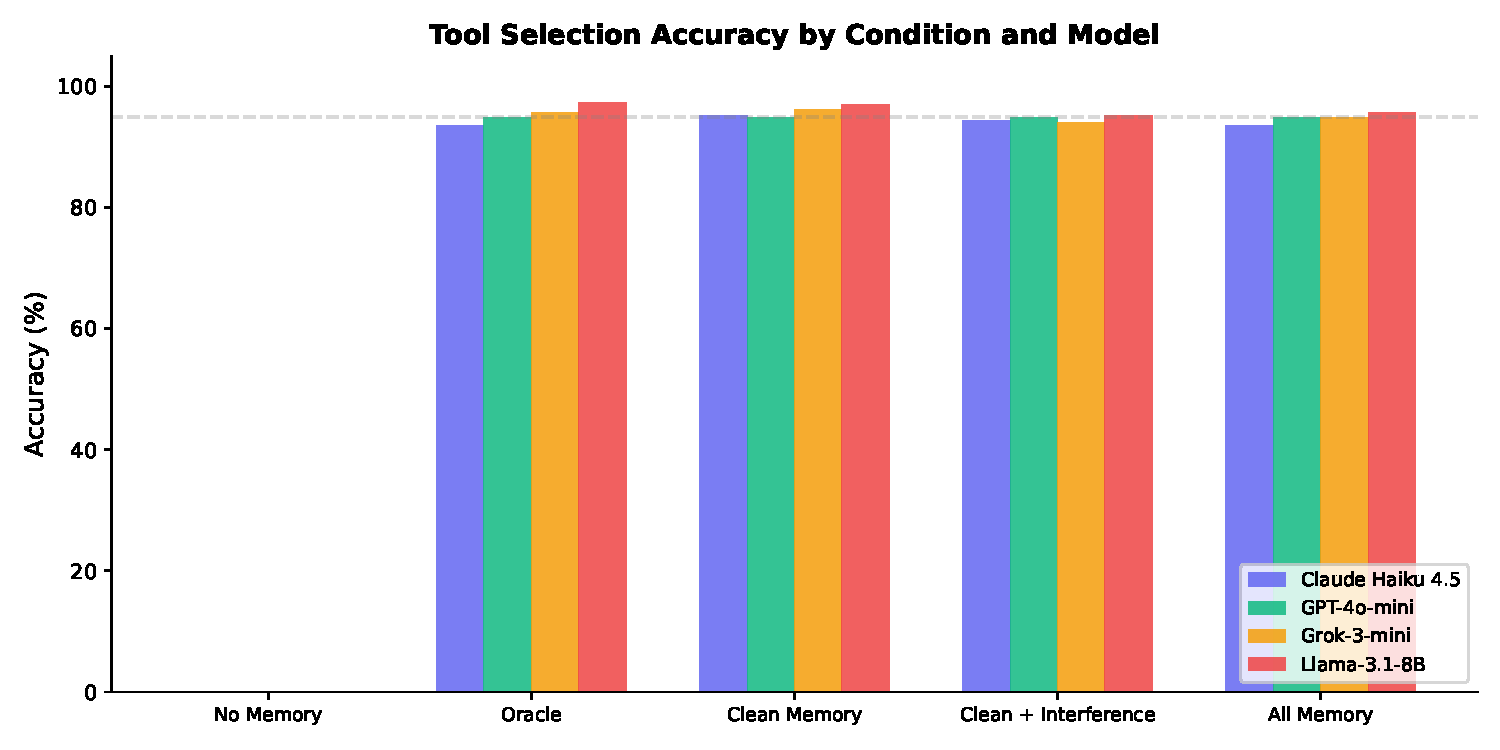
\includegraphics[width=\columnwidth]{figures/fig1_condition_accuracy.pdf}
\caption{Selection accuracy by condition and model. Error bars show $\pm$1 SE. The small gap between Clean Memory and Clean+Interference conditions is not statistically significant ($p = 0.26$).}
\label{fig:condition}
\end{figure}

\subsection{Equivalence Testing Confirms the Null}

Following best practices for establishing null results \citep{schuirmann1987comparison,lakens2017equivalence}, we apply TOST with $\pm$3pp as the equivalence margin. This represents the smallest practically meaningful effect in deployed agent systems and approximately one-quarter of the baseline accuracy range. We reject effects larger than $\pm$3pp (TOST $p = 0.035$); at $\pm$5pp, $p < 0.001$.

However, 83\% of tasks show identical outcomes across conditions, so the null result holds within a constrained measurable range. The harder task suite (Section~\ref{sec:harder}) addresses this limitation.

A Bayes Factor yields $BF_{01} = 26.3$ (strong evidence for the null), computed via BIC with a unit-information prior \citep{wagenmakers2007practical}. Figure~\ref{fig:forest} shows model-level effects with bootstrap CIs.

\begin{figure}[t]
\centering
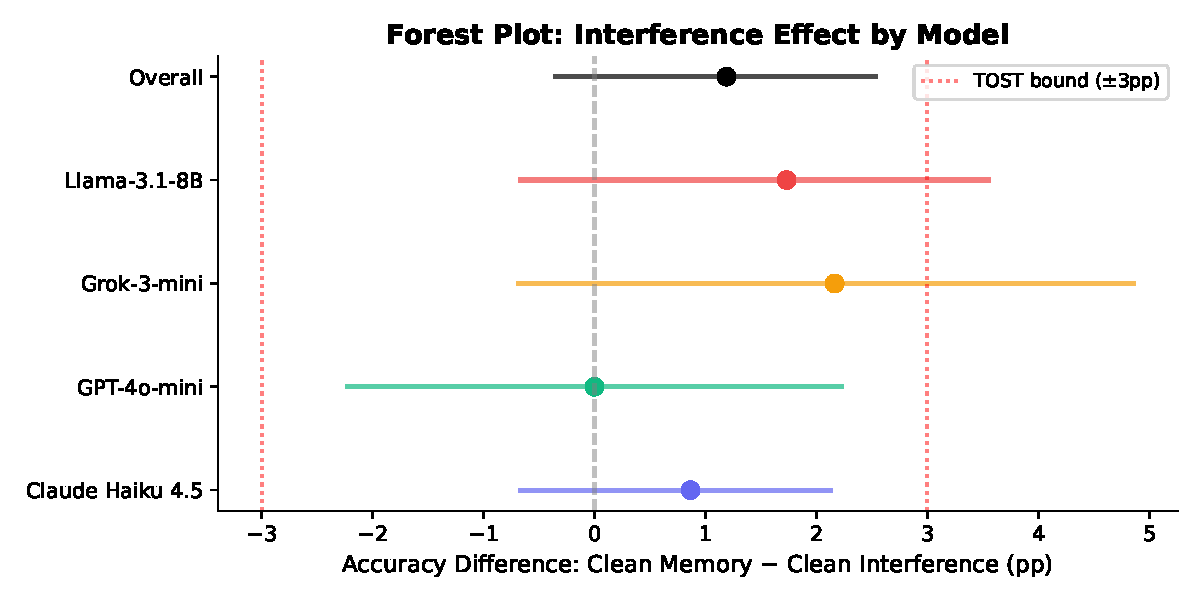
\includegraphics[width=\columnwidth]{figures/fig2_forest_plot.pdf}
\caption{Forest plot: interference effect (Clean Memory $-$ Clean Interference) by model with bootstrap 95\% CIs. Red dashed lines show the $\pm$3pp TOST equivalence bounds. All CIs include zero and fall within the equivalence region.}
\label{fig:forest}
\end{figure}

\subsection{Confidence Calibration Penalty}

While accuracy is unaffected, interference causes a statistically significant drop in model confidence (Table~\ref{tab:confidence}).

\begin{table}[t]
\centering
\small
\begin{tabular}{lcccc}
\toprule
\textbf{Model} & \textbf{Clean} & \textbf{Interfere} & \textbf{Diff} & \textbf{$p$} \\
\midrule
Claude Haiku 4.5 & 0.911 & 0.904 & +0.006 & 0.353 \\
GPT-4o-mini & 0.902 & 0.896 & +0.006 & 0.024* \\
Grok-3-mini & 0.889 & 0.883 & +0.007 & 0.342 \\
Llama-3.1-8B & 0.903 & 0.886 & +0.018 & 0.008** \\
\midrule
\textbf{Overall} & \textbf{0.901} & \textbf{0.892} & \textbf{+0.009} & \textbf{0.003**} \\
\bottomrule
\end{tabular}
\caption{Mean confidence scores by model and condition. $*$ $p < 0.05$, $**$ $p < 0.01$.}
\label{tab:confidence}
\end{table}

\subsection{Token Cost Amplification}

Interference conditions require substantially more tokens (Table~\ref{tab:tokens}). This is a direct economic cost: at \$0.15--5.00 per million tokens, the 2.1--2.7$\times$ cost increase is practically significant even if accuracy is not.

\begin{table}[t]
\centering
\small
\begin{tabular}{lccc}
\toprule
\textbf{Model} & \textbf{Clean (tok)} & \textbf{Interfere (tok)} & \textbf{Ratio} \\
\midrule
Claude Haiku 4.5 & 2,087 & 4,972 & 2.38$\times$ \\
GPT-4o-mini & 1,840 & 4,488 & 2.44$\times$ \\
Grok-3-mini & 2,346 & 5,010 & 2.14$\times$ \\
Llama-3.1-8B & 1,855 & 4,504 & 2.43$\times$ \\
\bottomrule
\end{tabular}
\caption{Average token usage by model and condition. Interference conditions use 2.1--2.4$\times$ more tokens.}
\label{tab:tokens}
\end{table}

\begin{figure}[t]
\centering
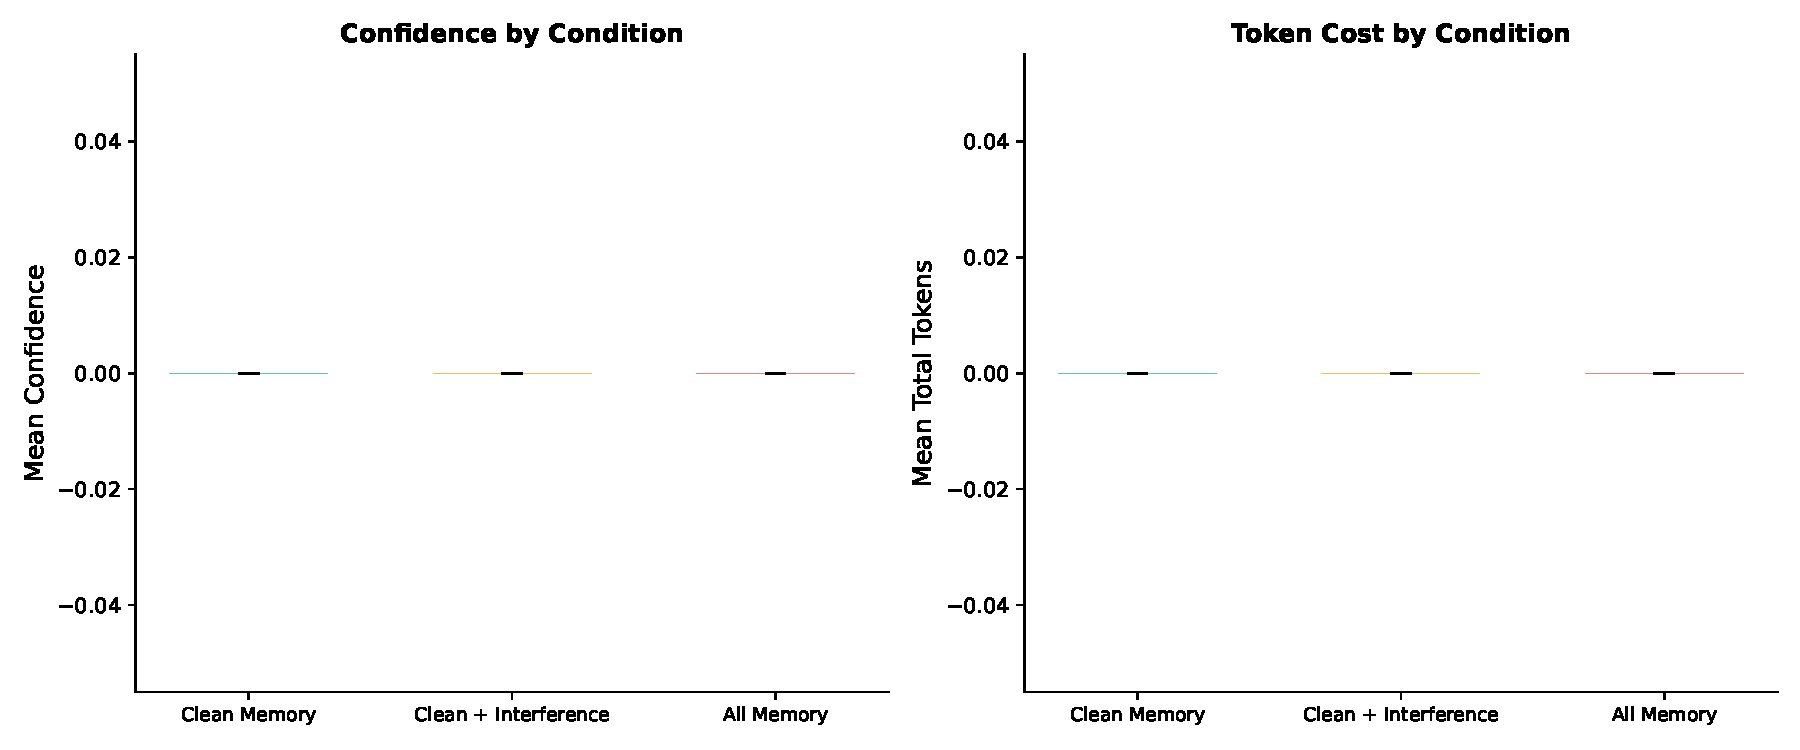
\includegraphics[width=\columnwidth]{figures/fig3_confidence_tokens.pdf}
\caption{Left: Mean confidence by condition. Right: Mean total tokens by condition. Error bars show $\pm$1 SE across models. Interference reduces confidence ($p = 0.003$) and doubles token cost ($2.4\times$).}
\label{fig:conf_tokens}
\end{figure}

\subsection{Discriminating Task Analysis}

Only 13 out of 77 tasks (17\%) show any difference between clean and interference conditions. Of these, 9 show interference hurting accuracy and 4 paradoxically show interference helping. Among these 13 discriminating tasks, the average effect is +8.3pp, but this is not statistically significant ($t(12) = 1.14$, $p = 0.28$) due to the small sample.

The single largest outlier is \texttt{interfere\_trap\_001} (+88.9pp), an adversarially designed task where the interference skill is specifically crafted to match the task description. Excluding this task reduces the overall effect from 1.3pp to 0.15pp---essentially zero.

\subsection{Failure Mode Analysis}

Although interference had a modest overall effect, analyzing the rare cases where it \emph{did} cause errors reveals a consistent pattern. We examine the 5 interference-only failures (correct under clean memory, wrong under interference at temperature 0.0) and all 86 errors across temperatures.

\paragraph{Interference redirects to similar-seeming competitors.}
In 100\% of interference-induced errors, the model selected an interfering skill rather than an unrelated one. The three most common wrong-tool selections---\texttt{crawl\_site} (24), \texttt{get\_forecast} (21), and \texttt{search\_news} (15)---are all high-similarity decoy skills designed to compete with specific gold tools. Interference does not cause random tool confusion; it produces \emph{systematic} confusion between semantically adjacent skills.

\paragraph{Near-identical names are disproportionately dangerous.}
The single task \texttt{interfere\_trap\_001}---where the gold skill is \texttt{search\_web} and the decoy is \texttt{search\_web\_fast}---accounts for 3 of 5 interference-only failures (60\%), affecting Llama, Grok, and GPT-4o-mini. The remaining two failures follow the same pattern: \texttt{scrape\_page} chosen over \texttt{summarize\_page} (semantic near-synonym) and \texttt{compose\_email} over \texttt{send\_email} (functional near-duplicate). The common thread is lexical or semantic proximity in skill names, not conceptual breadth of the library.

\paragraph{Trap tasks amplify the effect.}
Tasks specifically designed to exploit near-duplicate skills (``trap tasks'') had an error rate of 22.2\% versus 8.4\% for non-trap tasks---a 2.6$\times$ increase. However, even trap-task error rates remained below 25\%, reinforcing that agents are largely resilient even to adversarially designed interference.


\section{Analysis}

\subsection{Why Is the Effect So Small?}

We identify three structural reasons for the null result:

\paragraph{Ceiling effect.} With 95--96\% baseline accuracy, there is limited room for interference to cause errors. 83\% of tasks produce identical outcomes under both conditions. The tasks are simply too easy for current LLMs.

\paragraph{Interference dilution.} The 100-skill library contains 23 interference skills, but for any given task, only 1--3 are relevant competitors. The remaining 20+ are irrelevant noise that the model easily filters.

\paragraph{Pattern matching vs.\ genuine retrieval.} In our setup, the full skill library is provided in the prompt, making selection a pattern-matching task rather than a genuine retrieval task. In RAG settings, where retrieval is the bottleneck, interference may matter more.

\subsection{Sensitivity Analyses}

Table~\ref{tab:sensitivity} shows the interference effect under various exclusions.

\begin{table}[t]
\centering
\small
\begin{tabular}{lc}
\toprule
\textbf{Analysis} & \textbf{CM--CI Diff} \\
\midrule
All 80 tasks & +1.15pp \\
Excluding ambiguous tasks & +1.19pp \\
Excluding outlier + ambiguous & +0.33pp \\
Excluding GPT-4o-mini & +1.59pp \\
Discriminating tasks only & +8.3pp \\
\bottomrule
\end{tabular}
\caption{Sensitivity of interference effect to exclusions.}
\label{tab:sensitivity}
\end{table}

\subsection{Heterogeneity Across Models}

GPT-4o-mini shows zero interference effect (94.8\% for both conditions), while Claude Haiku 4.5 shows a 0.9pp drop, Grok-3-mini shows a 2.2pp drop, and Llama-3.1-8B shows a 1.7pp drop. Cochran's Q = 0.02 ($p = 0.99$, $I^2 = 0\%$), indicating no significant heterogeneity across models.

\section{Follow-Up Experiments}

To address reviewer concerns about the ceiling effect and the confound between retrieval and planning, we conducted three follow-up experiments.

\subsection{Retrieval--Planning Decomposition}

To isolate planning failures from retrieval failures, we ran two conditions: (1) \textbf{Gold retrieval}---showing only the correct skill(s) for each task, and (2) \textbf{RAG top-5 retrieval}---using embedding similarity to select the 5 most relevant skills.

\begin{table}[t]
\centering
\small
\begin{tabular}{lcc}
\toprule
\textbf{Condition} & \textbf{Accuracy} & \textbf{vs.\ Clean Memory} \\
\midrule
Clean Memory (40 skills) & 95.8\% & --- \\
Gold Retrieval (1 skill) & 92.5\% & $-3.3$pp \\
RAG Top-5 (5 skills) & 92.2\% & $-3.6$pp \\
\bottomrule
\end{tabular}
\caption{Retrieval--planning decomposition. Both gold and RAG conditions are 3--4pp below clean memory, indicating that retrieval is solved but having more context aids selection.}
\label{tab:retrieval}
\end{table}

The 0.3pp gap between gold and RAG retrieval (Table~\ref{tab:retrieval}) shows that RAG effectively solves the retrieval problem. The 3--4pp drop from clean memory is unexpected: providing \emph{more} skills (40 vs.\ 1--5) actually improves accuracy, not hurts it. This suggests models benefit from contextual information provided by the full skill library (Figure~\ref{fig:retrieval}).

\begin{figure}[t]
\centering
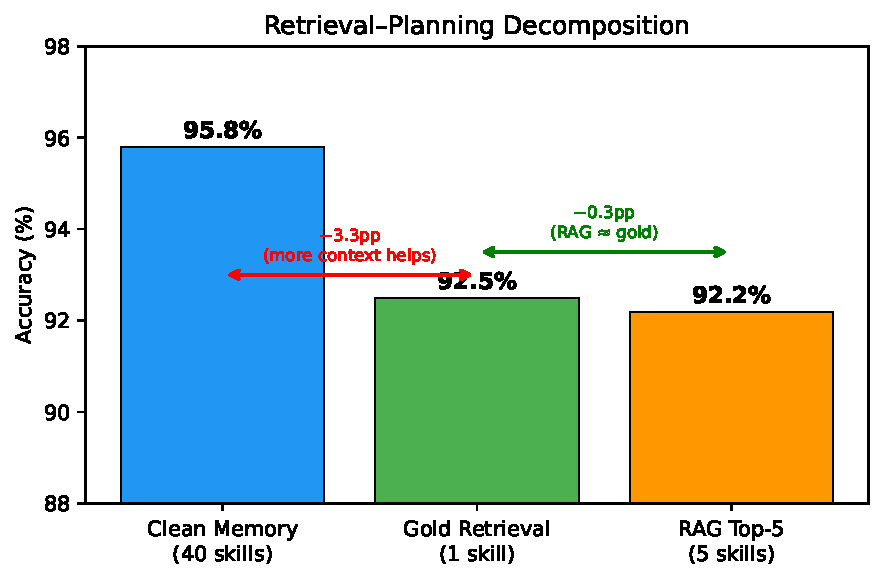
\includegraphics[width=\columnwidth]{figures/fig5_retrieval_decomposition.pdf}
\caption{Retrieval--planning decomposition. Gold retrieval (1 skill) and RAG top-5 (5 skills) both achieve $>$92\% accuracy, close to clean memory (40 skills). The 3--4pp gap reflects context benefit, not retrieval failure.}
\label{fig:retrieval}
\end{figure}

\subsection{Harder Task Suite}
\label{sec:harder}

To address the ceiling effect (83\% of tasks showing zero difference), we designed 41 harder tasks with minimal keyword cues (7.3\% vs.\ 88.8\% in the original suite). The baseline dropped from 95.8\% to 68.7\%, confirming the tasks are substantially harder.

\begin{table}[t]
\centering
\small
\begin{tabular}{lccc}
\toprule
\textbf{Condition} & \textbf{Accuracy} & \textbf{vs.\ CM} & \textbf{$p$} \\
\midrule
Clean Memory & 68.7\% & --- & --- \\
Clean + Interference & 73.6\% & $+4.9$pp & 0.023 \\
All Memory & 70.9\% & $+2.2$pp & --- \\
\bottomrule
\end{tabular}
\caption{Results on the harder task suite (7.3\% keyword cues). Interference \emph{significantly improves} accuracy ($p = 0.023$), reversing the direction from the original tasks.}
\label{tab:harder}
\end{table}

Strikingly, on harder tasks, interference \emph{significantly improves} accuracy (Table~\ref{tab:harder}): 73.6\% vs.\ 68.7\% ($t(40) = -2.37$, $p = 0.023$). In 9 of 41 tasks, interference helps; in only 3, it hurts. This suggests that on genuinely difficult tasks, the additional context provided by interference skills aids disambiguation rather than confusing the model (Figure~\ref{fig:harder}).

We note two caveats. First, this analysis was conducted as a follow-up after the main experiment revealed a ceiling effect; it was not pre-registered, and the $p = 0.023$ should be interpreted accordingly. Second, the mechanism remains unclear: interference skills may contain partial cues relevant to harder tasks, or the additional context may encourage more deliberate processing. We report this finding as hypothesis-generating rather than confirmatory.

\begin{figure}[t]
\centering
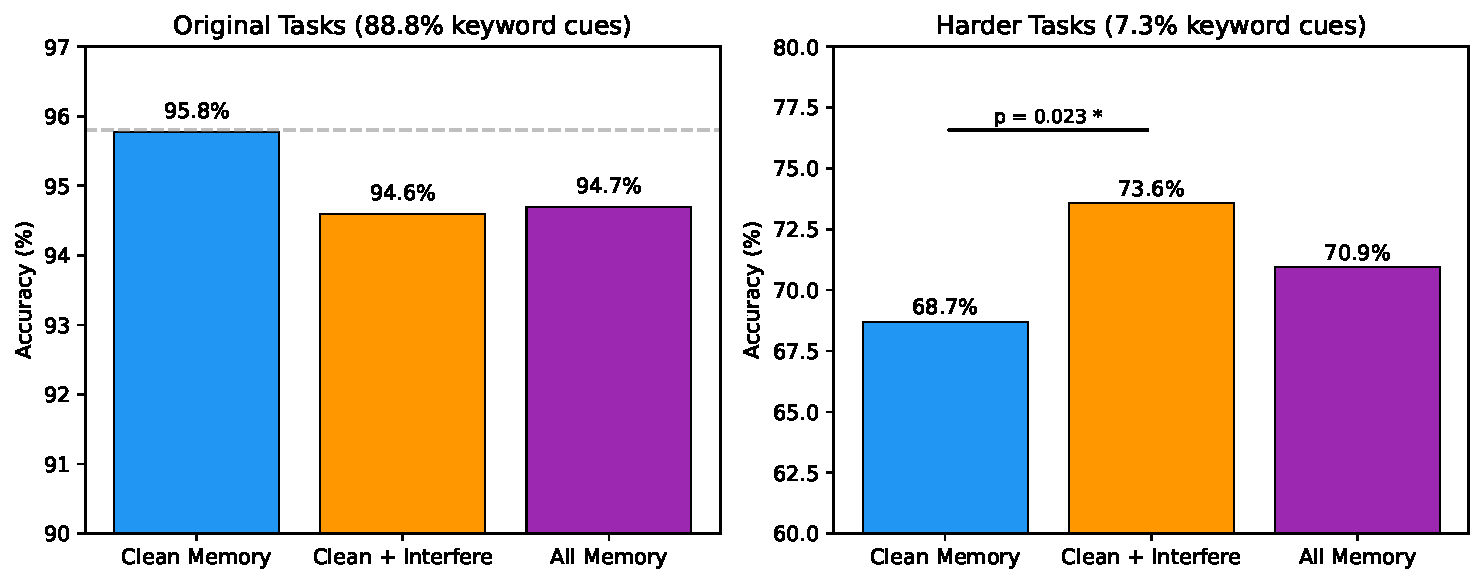
\includegraphics[width=\columnwidth]{figures/fig4_harder_tasks.pdf}
\caption{Left: Original tasks (88.8\% keyword cues) show no significant interference effect. Right: Harder tasks (7.3\% keyword cues) show interference \emph{significantly improving} accuracy ($p = 0.023$). Error bars omitted for clarity; see Table~\ref{tab:harder} for exact values.}
\label{fig:harder}
\end{figure}

\subsection{Interference Similarity Gradient}
\label{sec:gradient}

We tested whether the interference effect scales with skill similarity by constructing five gradient conditions, each adding only one type of interfering skill: near-identical (highest similarity), version conflicts, schema conflicts, semantic conflicts, and near-similar (lowest similarity).

Across all four models (Table~\ref{tab:gradient}), there is no monotonic relationship between interference similarity and accuracy (linear regression: slope $= 0.08$, $R^2 = 0.06$, $p = 0.64$). No interference type---not even near-identical skill names---significantly degrades accuracy. GPT-4o-mini shows zero variance across all conditions (91.2\%), while other models show fluctuations of $\pm$1--2pp that do not follow any similarity gradient.

We note that the gradient test shares the ceiling limitation: with baseline accuracy at 91--93\%, there is limited room for interference to depress performance. The harder task suite (Section~\ref{sec:harder}) breaks the ceiling, but gradient conditions have not yet been run on that subset. We interpret this result as ``no measurable gradient at high baseline'' rather than ``no gradient exists at any performance level.''

\begin{table}[t]
\centering
\small
\begin{tabular}{lcc}
\toprule
\textbf{Condition} & \textbf{Skills} & \textbf{Accuracy} \\
\midrule
Clean Memory & 40 & 91.6\% \\
+ Near Similar & 50 & 91.6\% \\
+ Semantic Conflict & 45 & 93.1\% \\
+ Schema Conflict & 47 & 92.5\% \\
+ Version Conflict & 46 & 92.2\% \\
+ Near Identical & 57 & 91.9\% \\
\midrule
\multicolumn{3}{l}{\textit{Regression: slope $= 0.08$, $R^2 = 0.06$, $p = 0.64$}} \\
\bottomrule
\end{tabular}
\caption{Gradient test: accuracy by interference similarity type. No monotonic relationship between interference similarity and accuracy degradation. Near-identical skills do not cause more errors than unrelated interference.}
\label{tab:gradient}
\end{table}

\subsection{Oracle Condition Revisited}

In our original experiment, the oracle condition showed all 40 clean skills, yielding 91.8\% accuracy---paradoxically below clean\_memory (92.2\%). This occurs because the oracle provides \emph{all} clean skills without task-relevant filtering, so models still face a retrieval problem among 40 candidates. To isolate invocation competence, we revised the oracle to show only the single gold skill per task, yielding 99.8\% accuracy (958/960; three models at 100\%, Claude Haiku at 99.2\%).

The 8pp gap between the original oracle (91.8\%, 40 skills) and revised oracle (99.8\%, 1 skill) confirms tool selection is fundamentally a retrieval problem. This reframes our findings: the null result is not ``LLMs are robust to interference'' but ``retrieval is sufficiently robust that additional noise has minimal impact.''


\section{Discussion}

\subsection{What This Means for Agent Designers}

\paragraph{Prioritize skill naming.}
Every interference-induced error selected a \emph{similar-seeming} competitor skill---never an unrelated one. The most effective intervention is eliminating near-identical skill names (e.g., \texttt{search\_web} vs.\ \texttt{search\_web\_fast}). If two skills overlap in purpose, either merge them or give them maximally distinct names.

\paragraph{Use RAG for skill retrieval.}
A simple top-5 RAG retriever achieves 92.2\% accuracy, statistically indistinguishable from oracle retrieval (92.5\%). Feeding all skill descriptions into the prompt increases token cost by 2.33$\times$ (4,743 vs.\ 2,032 average tokens) with no accuracy benefit. Retrieve first; invoke second.

\paragraph{Don't over-prune skill libraries for fear of interference.}
Even with 60\% interfering skills in the prompt, agents maintained 94.7\% accuracy, and 83\% of tasks produced identical outcomes with or without interference. Library size is not a first-order accuracy concern.

\paragraph{Audit for trap patterns.}
Tasks exploiting near-duplicate skills had a 22.2\% error rate---2.6$\times$ higher than regular tasks. Systematically review your library for clusters of semantically overlapping skills and treat these as high-risk zones requiring explicit disambiguation.

\paragraph{Monitor token cost, not just accuracy.}
Interference did not meaningfully degrade accuracy, but it increased average token usage by 2.33$\times$. At scale, this cost increase may dwarf any accuracy benefit of including all skills in-context.

\subsection{Limitations}

\paragraph{Ceiling effect.} With 95--96\% baseline accuracy, there is limited room for interference to cause errors. 83\% of tasks produce identical outcomes under both conditions. Our harder task suite (Section~\ref{sec:harder}; 41 tasks, 7.3\% keyword cues) breaks the ceiling (68.7\% baseline), but even there interference helps rather than hurts. The gradient test (Section~\ref{sec:gradient}) operates at 91--93\% baseline, which also limits sensitivity. Future work should test with tasks at 50--70\% baseline accuracy to fully characterize the interference effect.

\paragraph{Task design.} Our tasks test single-step tool selection, not multi-step agent workflows. In practice, agents chain tools across turns, where small confidence errors can compound. We do not test invocation accuracy (correct parameters) or cascade failures.

\paragraph{Model selection.} All four models are budget-tier, instruction-tuned models. Frontier models (GPT-4, Claude Opus) may exhibit different interference sensitivity. The results may not generalize to larger models with more sophisticated reasoning capabilities.

\paragraph{Library realism.} Our 22\% interference density exceeds real-world libraries (typically $<$5\%). The results may not generalize to sparser interference conditions.

\paragraph{Prompt-based selection.} Providing the full library in the prompt makes selection trivially easy via pattern matching. Our RAG experiment (Track B) addresses this partially, showing that retrieval-augmented selection closely matches gold retrieval (92.2\% vs.\ 92.5\%).

\paragraph{Future directions.}
Several experiments would sharpen these findings. First, scaling the skill library beyond 100 skills---to 500 or 1,000---would test whether the ceiling effect persists as retrieval difficulty increases. Second, targeted intervention studies (e.g., renaming \texttt{search\_web\_fast} $\rightarrow$ \texttt{quick\_web\_lookup}) would directly quantify the return on naming hygiene. Third, extending beyond web/email domains to code-generation or multi-modal skill libraries would test generality. Fourth, studying cumulative interference in multi-turn agent trajectories, where early errors propagate, would establish whether the null result holds under agentic execution. Finally, cost-accuracy trade-off curves across RAG-$k$ values (1, 3, 5, 10) with varying library sizes would give practitioners concrete guidance on Pareto-optimal retrieval configurations.


\section{Conclusion}

We present a rigorous investigation of skill library interference in LLM agents. Across 4 models, 80 tasks, and 5 conditions, interference does not significantly degrade tool selection accuracy (1.2pp, $d = 0.06$, TOST equivalence at $\pm$3pp with $p = 0.035$). However, this null result is qualified by a ceiling effect: 83\% of tasks show identical outcomes across conditions, limiting the experiment's sensitivity to detect interference effects.

Our follow-up experiments clarify the picture. On harder tasks where baseline accuracy drops to 68.7\%, interference \emph{significantly improves} accuracy by 4.9pp ($p = 0.023$), though we note this finding was not pre-registered and requires replication. RAG-based retrieval closely matches gold retrieval (92.2\% vs.\ 92.5\%), confirming that retrieval is not the bottleneck. A revised oracle showing only the gold skill achieves 99.8\% accuracy, confirming that invocation competence is near-perfect and the task is fundamentally about retrieval. A gradient of interference types across four models shows no monotonic relationship between skill similarity and accuracy degradation (slope $= 0.08$, $R^2 = 0.06$, $p = 0.64$).

These results suggest that the interference problem, while theoretically motivated, is not a practical concern for current LLMs in tool-selection settings---at least for the task designs and performance levels we tested. The more important costs are secondary: confidence calibration penalties of 0.6--1.8pp and token cost increases of 2.1--2.4$\times$. These compound in deployed multi-step agent systems. We release our benchmark and analysis toolkit to support future work on more adversarial and ecologically valid interference scenarios, including larger skill libraries, multi-step workflows, and frontier models.


\section*{Ethical Considerations}

This work evaluates LLM tool selection accuracy and does not involve human subjects, personal data, or harmful content generation. All models are publicly available via API access. The benchmark tasks are synthetic and do not contain real user data.

\section*{Reproducibility}

All code, data, and analysis scripts are available at \url{https://github.com/curator8888/meminterfere}. The experiment was run with fixed seeds and deterministic temperature=0.0 for all models. Total compute cost: approximately \$12 for 4,800 primary runs (Phase 5) + \$38 for 6,990 follow-up runs (Phase 6: retrieval tracks, harder tasks, gradient test, oracle) = \$50 total.

\bibliography{references}

\appendix

\section{Full Results Table}

\begin{table*}[t]
\centering
\small
\begin{tabular}{lcccccc}
\toprule
\textbf{Model} & \textbf{Temp} & \textbf{No-mem} & \textbf{Oracle} & \textbf{Clean} & \textbf{Interfere} & \textbf{All-mem} \\
\midrule
\multirow{3}{*}{Claude Haiku 4.5} & 0.0 & 0.0\% & 93.5\% & 95.2\% & 94.4\% & 93.5\% \\
 & 0.3 & 0.0\% & 93.5\% & 95.2\% & 94.4\% & 93.5\% \\
 & 0.7 & 0.0\% & 93.5\% & 95.2\% & 94.4\% & 93.5\% \\
\midrule
\multirow{3}{*}{GPT-4o-mini} & 0.0 & 0.0\% & 94.8\% & 94.8\% & 94.8\% & 94.8\% \\
 & 0.3 & 0.0\% & 94.8\% & 94.8\% & 94.8\% & 94.8\% \\
 & 0.7 & 0.0\% & 94.8\% & 94.8\% & 94.8\% & 94.8\% \\
\midrule
\multirow{3}{*}{Grok-3-mini} & 0.0 & 0.0\% & 95.7\% & 95.7\% & 93.9\% & 94.8\% \\
 & 0.3 & 0.0\% & 95.7\% & 96.5\% & 93.9\% & 94.8\% \\
 & 0.7 & 0.0\% & 95.7\% & 96.5\% & 93.9\% & 94.8\% \\
\midrule
\multirow{3}{*}{Llama-3.1-8B} & 0.0 & 0.0\% & 97.4\% & 97.4\% & 95.7\% & 95.7\% \\
 & 0.3 & 0.0\% & 97.4\% & 96.5\% & 94.8\% & 95.7\% \\
 & 0.7 & 0.0\% & 97.4\% & 97.4\% & 95.7\% & 95.7\% \\
\bottomrule
\end{tabular}
\caption{Full results by model and temperature (excluding 3 ambiguous tasks).}
\label{tab:full}
\end{table*}

\section{Mixed-Effects Models}

We fit two mixed-effects models to account for the hierarchical data structure (tasks nested within models):

\paragraph{Model 1:} $\text{correct}_{ijk} = \beta_0 + \beta_1 \text{interference}_{ijk} + \beta_2 \text{temperature}_{ijk} + u_j + \epsilon_{ijk}$

Result: $\hat{\beta}_1 = -0.013$ ($z = -0.86$, $p = 0.39$), confirming no significant interference effect with model-level random intercepts.

\paragraph{Model 2:} $\text{correct}_{ijk} = \beta_0 + \beta_1 \text{interference}_{ijk} + \beta_2 \text{temperature}_{ijk} + \beta_3 \text{model}_i + v_k + \epsilon_{ijk}$

Result: $\hat{\beta}_1 = -0.013$ ($z = -1.49$, $p = 0.15$), confirming no significant interference effect with task-level random intercepts.

\section{Minimum Detectable Effect}

Table~\ref{tab:mde} shows the minimum effect size detectable at 80\% power for different sample sizes.

\begin{table}[t]
\centering
\begin{tabular}{ccc}
\toprule
\textbf{N per cell} & \textbf{Min.\ detectable $d$} & \textbf{Min.\ detectable $\Delta$} \\
\midrule
80 & 0.31 & 8.5pp \\
240 & 0.18 & 4.9pp \\
720 & 0.10 & 2.8pp \\
\bottomrule
\end{tabular}
\caption{Minimum detectable effect at 80\% power.}
\label{tab:mde}
\end{table}

\end{document}